\chapter{Random Numbers}\label{S:RNG}

\begin{quote}
``Anyone who considers arithmetical methods of producing random digits is, of course, in a state of sin.'' --- John von Neumann (1951)
\end{quote}

\section{Physical Random Number Generators}\label{S:PhysRNG}
Physical devices such as the BINGO machine demonstrated in class can be used to produce an integer uniformly at random from a finite set of possibilities.  Such ``ball bouncing machines'' used in the British national lottery as well as the New Zealand LOTTO are complex nonlinear systems that are extremely sensitive to initial conditions (``chaotic'' systems) and are physical approximations of the probability model called a ``well-stirred urn'' or an equi-probable $\demoivre(1/k,\ldots,1/k)$ random variable.  

Let us look at the New Zealand LOTTO draws at \url{http://lotto.nzpages.co.nz/statistics.html} and convince ourselves that all fourty numbers $\{1,2,\ldots,39,40\}$ seem to be drawn uniformly at random.  The British lottery animation at \url{http://understandinguncertainty.org/node/39} shows how often each of the $49$ numbers came up in the first $1240$ draws.  Are these draws really random?  We will answer these questions in the sequel (see \url{http://understandinguncertainty.org/node/40} if you can't wait).

\section{Pseudo-Random Number Generators}\label{S:RNGIntro}
Our probability model and the elementary continuous $\uniform(0,1)$ RV are built from the abstract concept of a random variable over a probability triple.  A direct implementation of these ideas on a computing machine is not possible. In practice, random variables are typically simulated by {\bf deterministic} methods or algorithms.  Such algorithms generate sequences of numbers 
whose behavior is virtually indistinguishable from that of truly random 
sequences.  In computational statistics, simulating realisations from a given RV is usually done in two distinct steps.  First, sequences of numbers that imitate  independent and identically distributed (IID) $\uniform(0,1)$ RVs are generated.  Second, appropriate transformations are made to these imitations of IID $\uniform(0,1)$ random variates in order to imitate IID random variates from other random variables or other random structures.  These two steps are essentially independent and are studied by two non-overlapping groups of researchers.  The formal term {\bf pseudo-random number generator} (PRNG) or simply {\bf random number generator} (RNG) usually
refers to some deterministic algorithm used in the first step to produce pseudo-random numbers (PRNs) that imitate IID $\uniform(0,1)$ random variates.

In the following chapters, we focus on transforming IID $\uniform(0,1)$ variates to other non-uniform variates.  In this chapter, we focus on the art of imitating IID $\uniform(0,1)$ variates using simple deterministic rules.  

\subsection{Linear Congruential Generators}\label{S:RNGs}

The following procedure introduced by D.~H.~Lehmer in 1949 [{\em Proc.~2nd Symp.~on Large-Scale Digital Calculating Machinery, Harvard Univ.~Press, Cambridge, Mass., 1951, 141--146}] gives the simplest popular PRNG that can be useful in many statistical situations if used wisely.

\begin{algorithm}[htpb]
\caption{Linear Congruential Generator (LCG)}
\label{AL:LCG}
\begin{algorithmic}[1]
\STATE{ {\it input:} five {\em suitable} integers:
\begin{enumerate}
\item $m$, the modulus; $0 < m$
\item $a$, the multiplier; $0 \leq a < m$
\item $c$, the increment; $0 \leq c < m$
\item $x_0$, the seed; $0 \leq x_0 < m$
\item $n$, the number of desired pseudo-random numbers
\end{enumerate}
}
\STATE {{\it output:} $(x_0,x_1,\ldots,x_{n-1})$, the linear congruential sequence of length $n$}
\FOR{$i=1$ to $n-1$}
\STATE $x_i \gets (a x_{i-1} + c) \mod m$
\ENDFOR
\STATE{{\it return:}  $(x_1,x_2,\ldots,x_n)$}
\end{algorithmic}
\end{algorithm}

In order to implement LCGs we need to be able to do high precision exact integer arithmetic in {\sc Matlab}.  We employ the Module {\tt vpi} to implement variable precision integer arithmetic.  You need to download this module for the next Labwork.

\begin{labwork}[Generic Linear Congruential Sequence]\label{LW:GenericLCGS}
Let us implement Algorithm~\ref{AL:LCG} in {\sc Matlab} as follows.
\VrbMf[label=LinConGen.m]{scripts/LinConGen.m}
We can call it for some arbitrary input arguments as follows:
\begin{VrbM}
>> LinConGen(13,12,11,10,12)
ans =    10     1    10     1    10     1    10     1    10     1    10     1
>> LinConGen(13,10,9,8,12)
ans =     8    11     2     3     0     9     8    11     2     3     0     9
\end{VrbM}
and observe that the generated sequences are not ``random'' for input values of $(m,a,c,x_0,n)$ equalling $(13,12,11,10,12)$ or $(13,10,9,8,12)$.  Thus, we need to do some work to determine the {\em suitable} input integers $(m,a,c,x_0,n)$.
\end{labwork}

\begin{labwork}[LCG with period length of $32$]\label{LW:LinConGenKnuth334T1L5}
Consider the linear congruential sequence with $(m,a,c,x_0,n)=(256,137,0,123,257)$ with period length of only $32 < m=256$.  We can visualise the sequence as plots in Figure~\ref{F:LinConGenKnuth334T1L5Plots} after calling the following M-file.
\VrbMf[label=LinConGenKnuth334T1L5Plots.m]{scripts/LinConGenKnuth334T1L5Plots.m}
\end{labwork}

\begin{figure}[htbp]
\caption{The linear congruential sequence of {\tt LinConGen(256,137,0,123,257)} with non-maximal period length of $32$ as a line plot over $\{0,1,\ldots,256\}$, scaled over $[0,1]$ by a division by $256$ and a histogram of the $256$ points in $[0,1]$ with $15$ bins.\label{F:LinConGenKnuth334T1L5Plots}}
\centering   \makebox{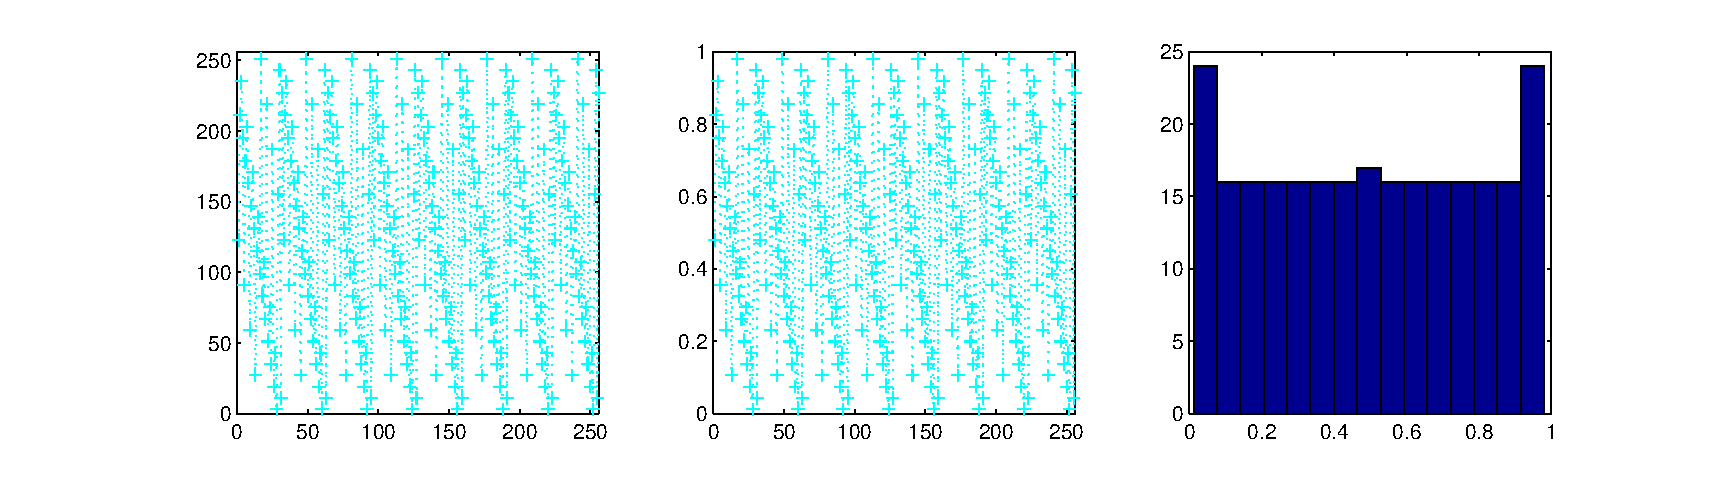
\includegraphics[width=7.0in]{figures/LinConGenKnuth334T1L5Plots}}
\end{figure}


\subsubsection*{Choosing the {\em suitable} magic input $(m,a,c,x_0,n)$}

The linear congruential  generator is a special case of a {\em discrete dynamical system}: 
\[
x_{i}  = f(x_{i-1}), \ f: \{0,1,2,\ldots,m-1\} \to \{0,1,2,\ldots,m-1\} \ \text{and} \ f(x_{i-1})=(a x_{i-1} + c) \mod m\enspace .
\]  
Since $f$ maps a the finite set $\{1,2,\ldots,m-1\}$ into itself, such systems are bound to have a repeating cycle of numbers called the {\bf period}.  In Labwork~\ref{LW:GenericLCGS}, the generator {\tt LinConGen(13,12,11,10,12)} has period $(10,1)$ of length $2$, the generator {\tt LinConGen (13,10,9,8,12)} has period $(8, 11, 2, 3, 0, 9)$ of length $6$ and the generator {\tt LinConGen(256,137,0,123,257)} has a period of length $32$.  All these generators have a non-maximal period length less than their modulus $m$.  A good generator should have a maximal period of $m$.  Let us try to implement a generator with a maximal period of $m=256$.


The period of a general LCG is at most $m$, and for some choices of $a$ the period can be much less than $m$ as shown in the examples considered earlier.  The LCG will have a full period if and only if:
\begin{enumerate}
\item $c$ and $m$  are relatively prime,
\item  $a-1$ is divisible by all prime factors of $m$,
\item  $a-1$ is a multiple of $4$ if  $m$ is a multiple of $4$
\end{enumerate}

\begin{labwork}[LCG with maximal period length of $256$]
Consider the linear congruential sequence with $(m,a,c,x_0,n)= (256,137,123,13,256)$.  First check that these parameters do indeed satisfy the three condition above and therefore can produce the maximal period length of only $m=256$.  Modify the input parameter to {\tt LinConGen} and repeat Labwork~\ref{LW:LinConGenKnuth334T1L5} in order to first produce a sequence of length $257$.  Do you see that the period is of maximal length of $256$ as opposed to the generator of Labwork~\ref{LW:LinConGenKnuth334T1L5}?  Next produce a Figure to visualise the sequence as done in Figure~\ref{F:LinConGenKnuth334T1L5Plots}.
\end{labwork}

A useful sequence should clearly have a relatively long period, say at least $2^{30}$.  Therefore, the {\bf modulus $m$ has to be rather large} because the {\bf period} cannot have more than $m$ elements.  Moreover, the quality of pseudo-random numbers of a LCG is extremely sensitive to the choice of $m$, $a$ and $c$ even if the maximal period is attained.  The next example illustrates this point.

\begin{labwork}[The infamous {\tt RANDU}]\label{LW:RANDU}
{\tt RANDU} is an infamous LCG, which has been used since the 1960s.  It is widely considered to be one of the most ill-conceived random number generators designed. Notably, it fails the {\bf spectral test} badly for dimensions greater than 2.  The following commands help visualise the sequence of first $5001/3$ triplets $(x_i,x_{i+1},x_{i+2})$ seeded from $x_0=1$ (Figure~\ref{F:RANDU3D5001pts}).  Read {\tt help reshape} and {\tt help plot3}. 
\begin{VrbM}
>> x=reshape( (LinConGen(2147483648,65539,0,1,5001)./ 2147483648) ,3,[]);
>> plot3(x(1,:),x(2,:),x(3,:),'.')
\end{VrbM}
\end{labwork}

\begin{figure}[htbp]
\caption{The LCG called {\tt RANDU} with $(m,a,c)=(2147483648,65539,0)$ has strong correlation between three consecutive points as: $x_{i+2}=6x_{k+1}-9x_k$.  The two plots are showing $(x_i,x_{i+1},x_{i+2})$ from two different view points.
.\label{F:RANDU3D5001pts}}
\centering   \makebox{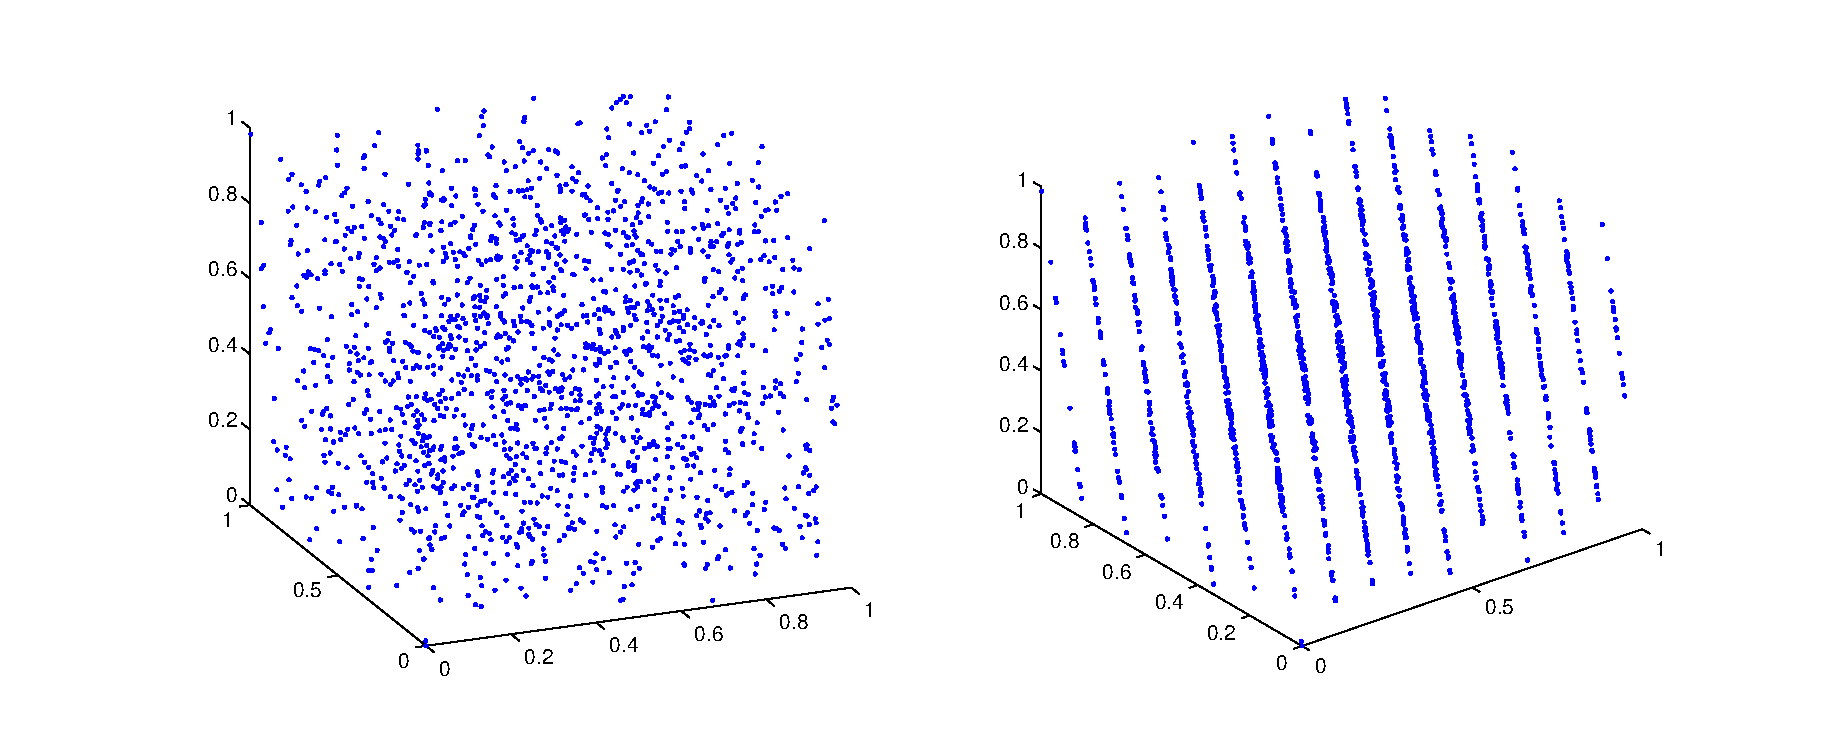
\includegraphics[width=7.0in]{figures/RANDU3D5001pts}}
\end{figure}

\begin{labwork}[Fishman20 and Lecuyer21 LCGs]
The following two LCGs are recommended in Knuth's Art of Computer Programming, vol.~2, for generating pseudo-random numbers for simple simulation tasks.
\begin{VrbM}
>> LinConGen(2147483647,48271,0,08787458,10) ./ 2147483647
ans =    0.0041    0.5239    0.0755    0.7624    0.6496    0.0769    0.9030    0.4259    0.9948    0.8868

>> LinConGen(2147483399,40692,0,01234567,10) ./ 2147483399
ans =    0.0006    0.3934    0.4117    0.7893    0.3913    0.6942    0.6790    0.3337    0.2192    0.1883
\end{VrbM}
\end{labwork}

The number of random numbers $n$ should at most be about $m/1000$ in order to avoid the future sequence from behaving like the past.  Thus, if $m=2^{32}$ then a new generator, with a new suitable set of $(m,a,c,x_0,n)$ should be adopted after the consumption of every few million pseudo-random numbers.

The LCGs are the least sophisticated type of PRNGs.  They are easier to understand but are not recommended for intensive simulation purposes.  The next section briefly introduces a more sophisticated PRNG we will be using in this course.  Moreover our implementation of LCGs using the variable precision integer package is extremely slow in {\sc MATLAB} and is only of pedagogical interest. 

\subsection{Generalized Feedback Shift Register  and the``Mersenne Twister'' PRNG} 

The following generator termed {\tt twister} in {\sc Matlab} is recommended for use in simulation.  It has extremely long periods, low correlation and passes most statistical tests (the {\sc diehard} statistical tests).  The {\tt twister} random number generator of Makoto Matsumoto and Takuji Nishimura is a variant of the twisted generalized feedback shift-register algorithm, and is known as the ``Mersenne Twister'' generator [Makoto Matsumoto and Takuji Nishimura, {\em Mersenne Twister: A 623-dimensionally equidistributed uniform pseudorandom number generator}, ACM Transactions on Modeling and Computer
Simulation, Vol.~8, No.~1 (Jan.~1998), Pages 3--30].  It has a Mersenne prime period of $2^{19937} - 1$ (about $10^{6000}$) and is {\bf equi-distributed} in $623$ dimensions.  It uses $624$ words of state per generator and is comparable in speed to the other generators.  The recommended default seed is $5489$.  See \url{http://www.math.sci.hiroshima-u.ac.jp/~m-mat/MT/emt.html} and \url{http://en.wikipedia.org/wiki/Mersenne_twister} for details.  

Let us learn to implement the {\sc Matlab} function that generates PRNs.  In {\sc Matlab} the function {\tt rand} produces a deterministic PRN sequence.  First, read {\tt help rand}.  We can generate PRNs as follows.
\begin{labwork}[Calling PRNG in {\sc Matlab}]\label{LW:RNGMatlab}
In {\sc Matlab} {\tt rand} is basic PRNG command.
\begin{VrbM}
>> rand(1,10) % generate a 1 X 10 array of PRNs
ans =
    0.8147    0.9058    0.1270    0.9134    0.6324    0.0975    0.2785    0.5469    0.9575    0.9649
>> rand(1,10) % generate another 1 X 10 array of PRNs
ans =
    0.1576    0.9706    0.9572    0.4854    0.8003    0.1419    0.4218    0.9157    0.7922    0.9595
>> rand('twister',5489) % reset the PRNG to default state Mersenne Twister with seed=5489
>> rand(1,10) % reproduce the first array
ans =
    0.8147    0.9058    0.1270    0.9134    0.6324    0.0975    0.2785    0.5469    0.9575    0.9649
>> rand(1,10) % reproduce the second array
ans =
    0.1576    0.9706    0.9572    0.4854    0.8003    0.1419    0.4218    0.9157    0.7922    0.9595
\end{VrbM}  
In general, you can use any seed value to initiate your PRNG.  You may use the {\tt clock} command to set the seed:
\begin{VrbM}
>> SeedFromClock=sum(100*clock); % save the seed from clock
>> rand('twister',SeedFromClock) % initialize the PRNG
>> rand(1,10)
ans =
    0.3696    0.3974    0.6428    0.6651    0.6961    0.7311    0.8982    0.6656    0.6991    0.8606
>> rand(2,10)
ans =
    0.3432    0.9511    0.3477    0.1007    0.8880    0.0853    0.6067    0.6976    0.4756    0.1523
    0.5827    0.5685    0.0125    0.1555    0.5551    0.8994    0.2502    0.5955    0.5960    0.5700
>> rand('twister',SeedFromClock) % initialize the PRNG to same SeedFromClock
>> rand(1,10)
ans =
    0.3696    0.3974    0.6428    0.6651    0.6961    0.7311    0.8982    0.6656    0.6991    0.8606
\end{VrbM}
\end{labwork}
 
\begin{figure}[htbp]
\caption{Triplet point clouds from the ``Mersenne Twister'' with two different seeds (see Labwork~\ref{LW:3DPlotsMersenneTwister}).
.\label{F:MersenneTwisterTwo3DPtclouds}}
\centering   \makebox{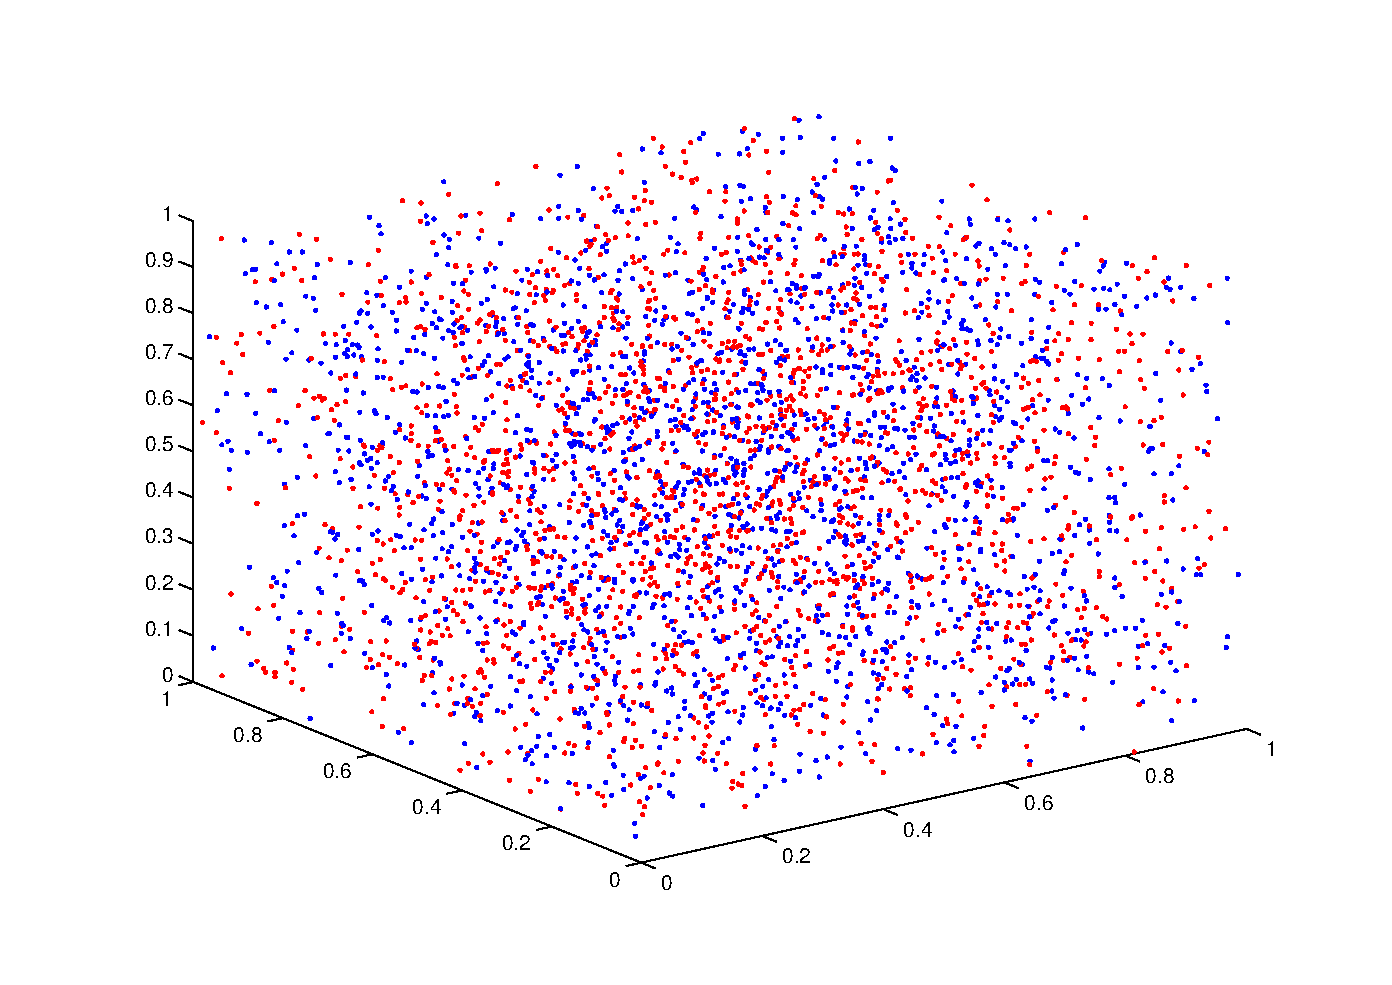
\includegraphics[width=6.0in]{figures/MersenneTwisterTwo3DPtclouds}}
\end{figure}
\begin{labwork}[3D plots of triplets generated by the ``Mersenne Twister'']\label{LW:3DPlotsMersenneTwister}
Try to find any correlation between triplets generated by the ``Mersenne Twister'' by rotating the 3D plot generated by the following code:
\begin{VrbM}
>> rand('twister',1234)
>> x=rand(3,2000); % store PRNs in a 3X2000 matrix named x
>> plot3(x(1,:),x(2,:),x(3,:),'.')
\end{VrbM}
Compare this with the 3D plot of triplets from {\tt RANDU} of Labwork~\ref{LW:RANDU}. Which of these two PRNGs do you think is ``more random'' looking? and why? 

Change the seed value to the recommended default by the authors and look at the point cloud (in red) relative to the previous point cloud (in blue).  Rotate the plots to visualise from multiple angles.  Are they still random looking?
\begin{VrbM}
>> rand('twister',1234)% same seed as before
>> x=rand(3,2000); % store PRNs in a 3X2000 matrix named x
>> rand('twister',5489)% the recommended default seed
>> y=rand(3,2000);% store PRNs seeded by 5489 in a 3X2000 matrix named y
>> plot3(x(1,:),x(2,:),x(3,:),'b.') % plot triplets as blue dots
>> hold on;
>> plot3(y(1,:),y(2,:),y(3,:),'r.') % plot triplets as red dots
\end{VrbM}
\end{labwork}
